
\documentclass[11pt]{article}
\usepackage{latexsym}
\usepackage{amsmath}
\usepackage{amssymb}
\usepackage{amsthm}
\usepackage{epsfig}
\usepackage{lipsum}
\usepackage{graphicx}
\usepackage{algorithm,float}
%\usepackage{algorithmic}
\usepackage[noend]{algpseudocode}
\usepackage{algorithm}% http://ctan.org/pkg/algorithms
\MakeRobust{\Call}
\theoremstyle{definition}
\newtheorem{exmp}{Example}[section]

\newcommand{\handout}[5]{
  \noindent
  \begin{center}
  \framebox{
    \vbox{
      \hbox to 5.78in { {\bf ICS 621: Analysis of Algorithms } \hfill #2 }
      \vspace{4mm}
      \hbox to 5.78in { {\Large \hfill #5  \hfill} }
      \vspace{2mm}
      \hbox to 5.78in { {\em #3 \hfill #4} }
    }
  }
  \end{center}
  \vspace*{4mm}
}

\newcommand{\lecture}[4]{\handout{#1}{#2}{#3}{Scribe: #4}{Lecture #1}}

\newtheorem{theorem}{Theorem}
\newtheorem{corollary}[theorem]{Corollary}
\newtheorem{lemma}[theorem]{Lemma}
\newtheorem{observation}[theorem]{Observation}
\newtheorem{proposition}[theorem]{Proposition}
\newtheorem{definition}[theorem]{Definition}
\newtheorem{claim}[theorem]{Claim}
\newtheorem{fact}[theorem]{Fact}
\newtheorem{assumption}[theorem]{Assumption}

% 1-inch margins, from fullpage.sty by H.Partl, Version 2, Dec. 15, 1988.
\topmargin 0pt
\advance \topmargin by -\headheight
\advance \topmargin by -\headsep
\textheight 8.9in
\oddsidemargin 0pt
\evensidemargin \oddsidemargin
\marginparwidth 0.5in
\textwidth 6.5in

\parindent 0in
\parskip 1.5ex
%\renewcommand{\baselinestretch}{1.25}
% for whole paragraph indent
\newenvironment{myindentpar}[1]%
  {\begin{list}{}%
          {\setlength{\leftmargin}{#1}}%
          \item[]%
  }
  {\end{list}}




\begin{document}

\lecture{5}{Fall 2019}{Prof.\ Nodari Sitchinava}{Honggen Zhang, Mojtaba Abolfazli, Sushil Shrestha}

% \section{Overview}
\section{Search Trees}
    \subsection{Binary Search Trees}
        Each node of a binary search tree requires at least a variable to store key, left child pointer, right child pointer and possibly parent pointer. Binary search trees can be implemented in C programming language using:

    \begin{verbatim}
struct Node{
    int key;
    Node *left;
    Node *right;
    Node *parent;
}

Node tree[totalNodes];
    \end{verbatim}

    We can use an array of \emph{Node} objects to store all the vertices in a binary tree. These data structures are stored sequentially in memory and can be represented as in Figure \ref{fig:structrepresentation}.
    \begin{figure}[tbh]
        \centering
        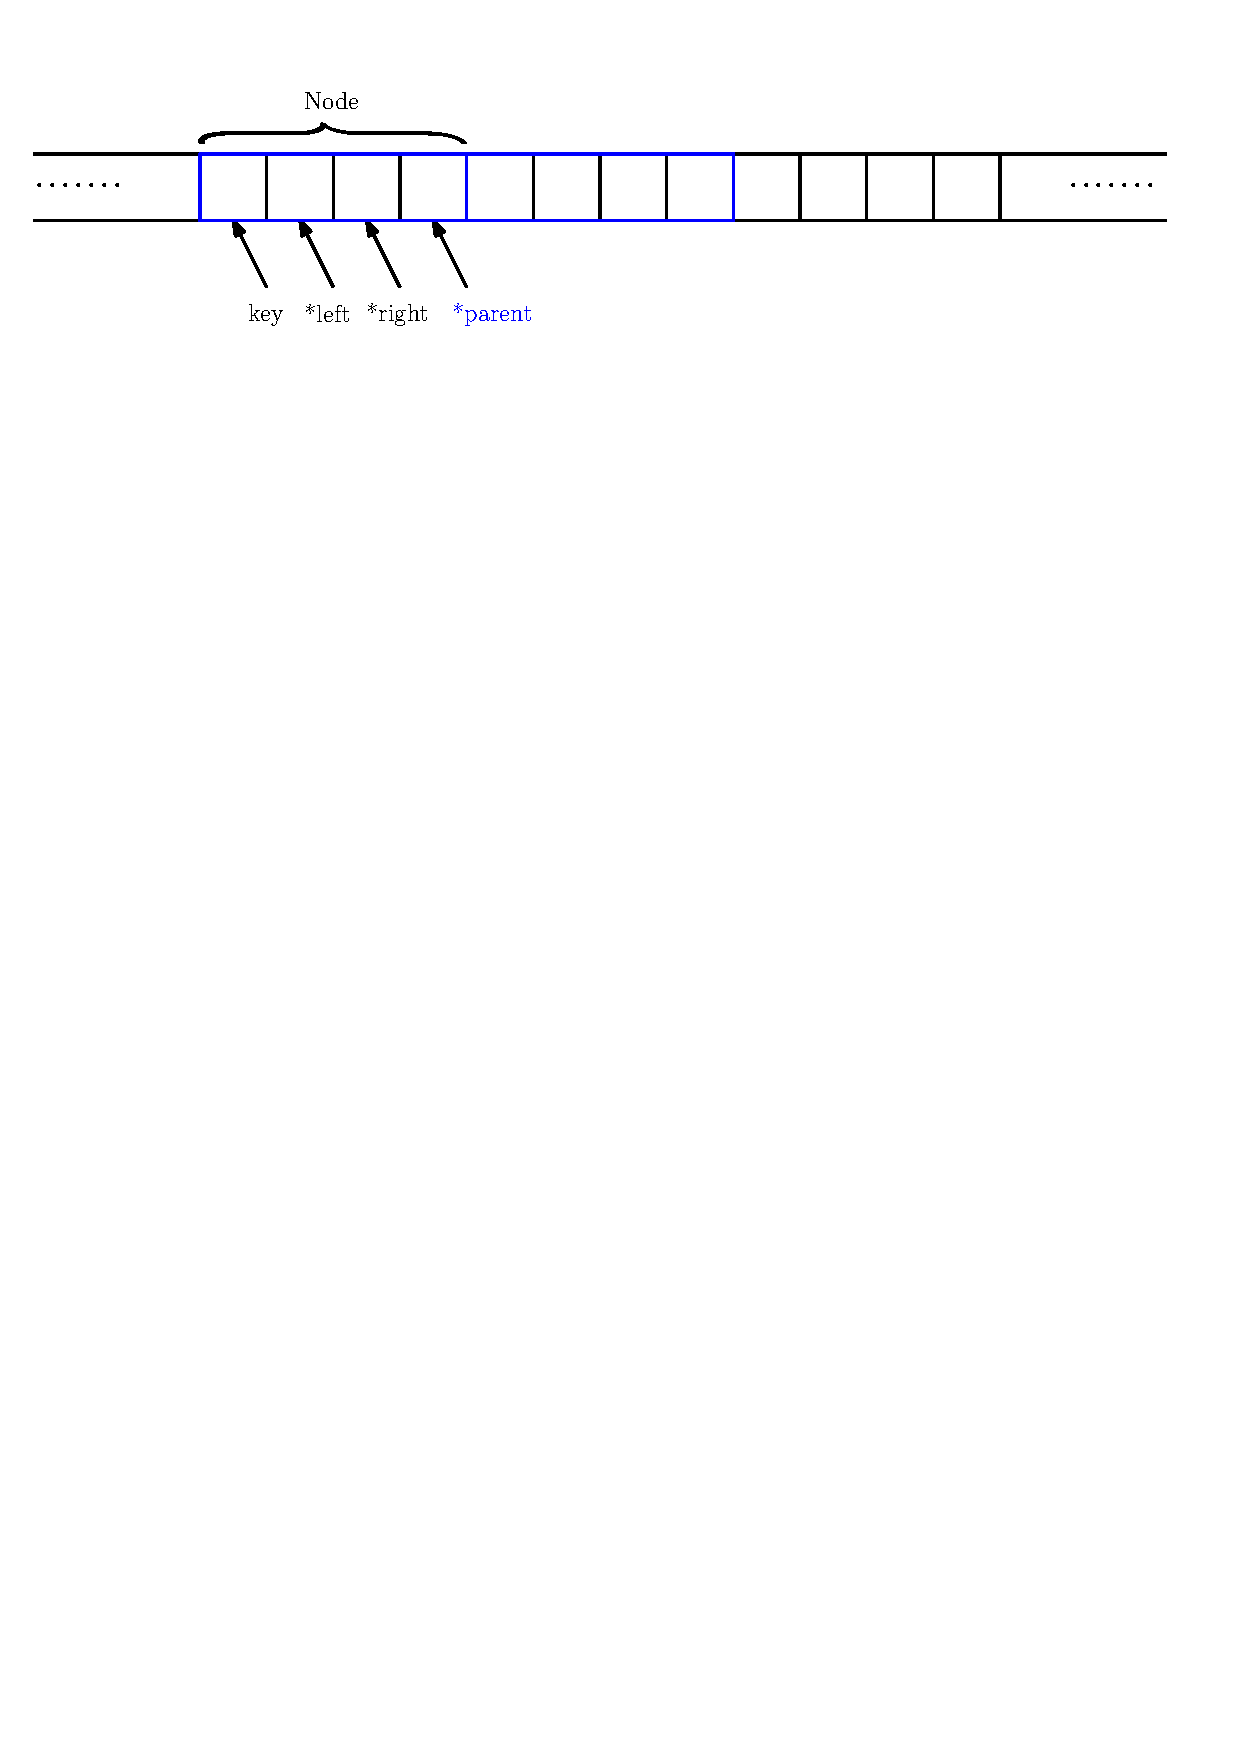
\includegraphics[scale=0.7]{struct-representation.pdf}
        \caption{Struct representation in memory.}
        \label{fig:structrepresentation}
    \end{figure}

    If we want to implement a binary search tree in a programming language that doesn't include the feature of struct or pointers, we can implement the same thing using 4 separate arrays to get the same feature as we have in our C implementation.
    \begin{figure}[tbh]
        \centering
        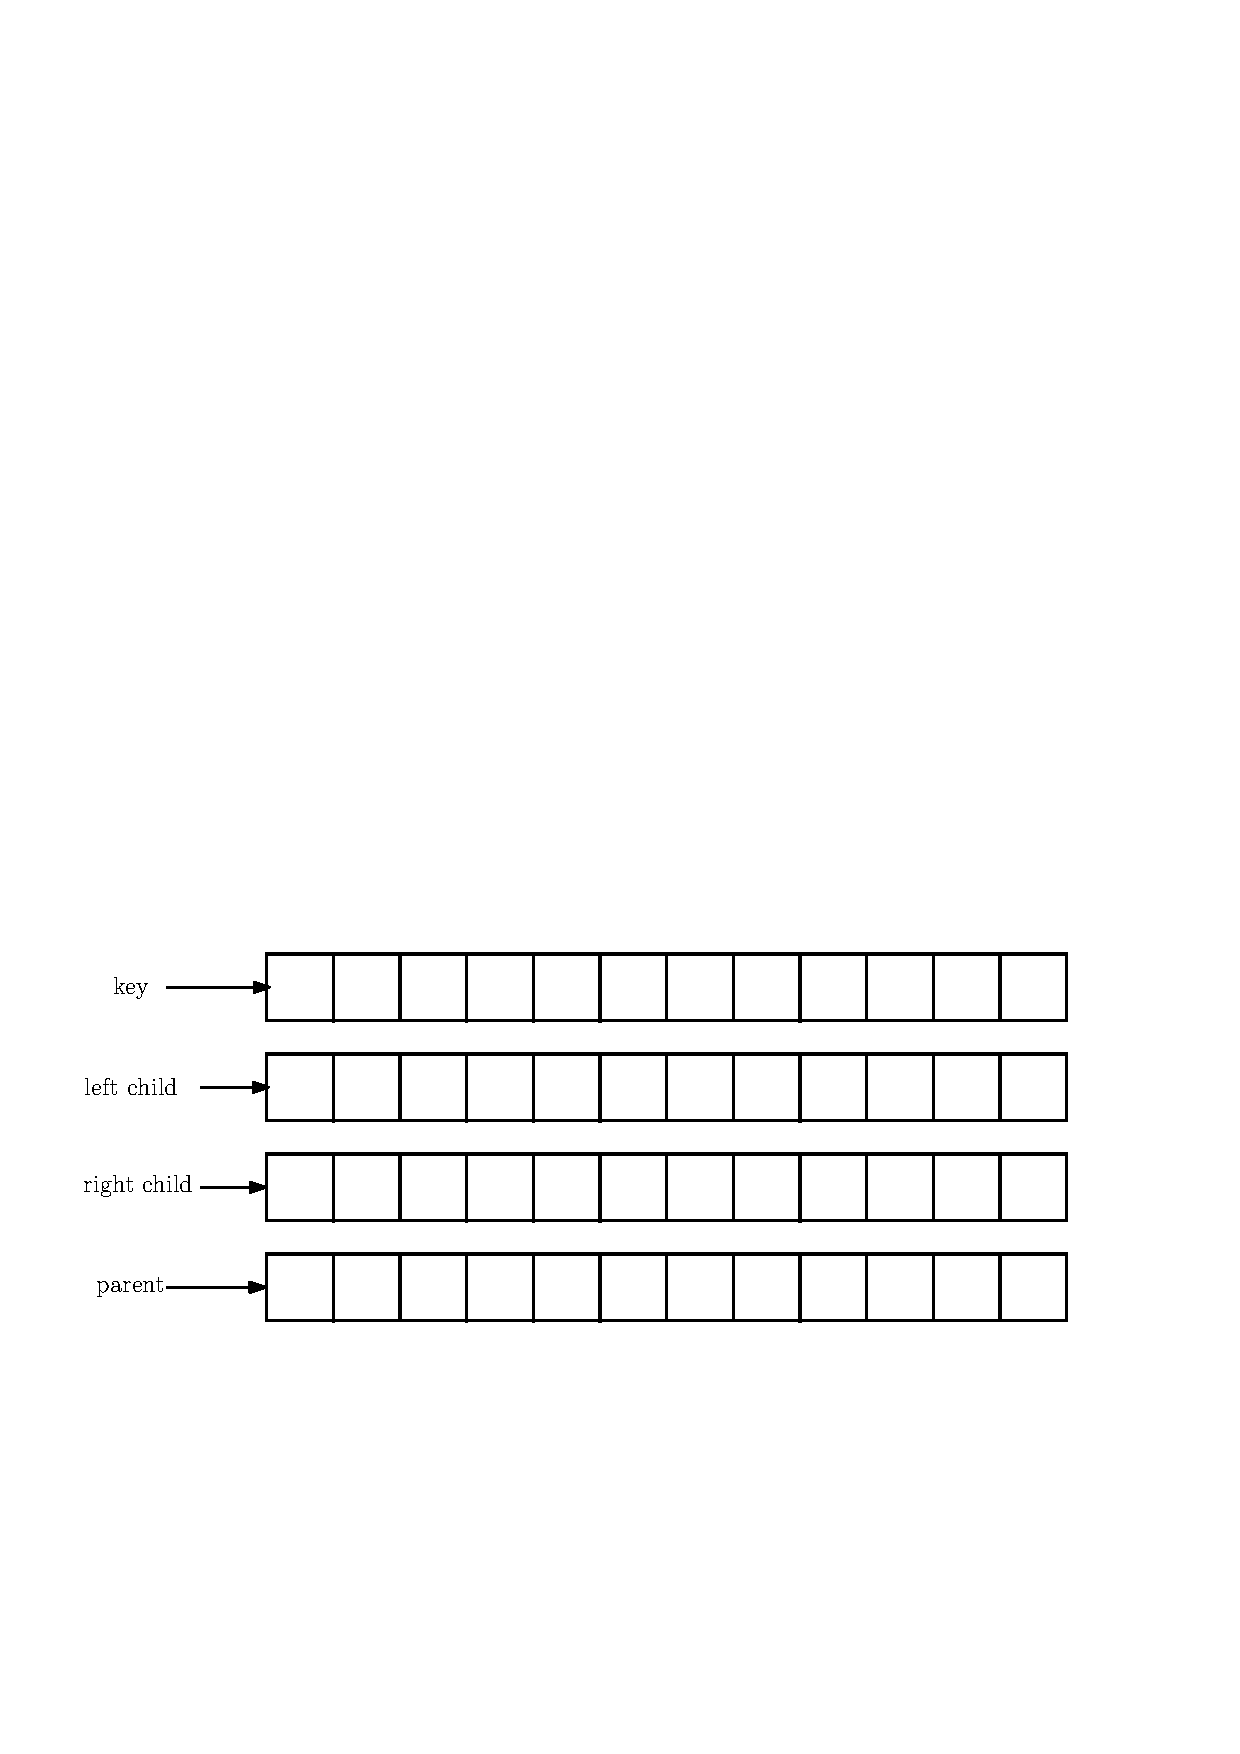
\includegraphics[scale=0.8]{arrayrepresentation.pdf}
        \caption{Array representation of binary tree}
        \label{fig:arrayrepresentation}
    \end{figure}

    Both of the representations are identical except for the case when we consider caching effects on our data structure.

    \subsection*{Balanced binary search tree}
    The cost of searching for an item in a balanced binary search tree is $\Theta(\log{(n)})$. Balanced binary tree can be maintained by rearranging the tree after certain number of inserts to the binary search tree.
    
    \begin{algorithm}[H]
        \caption{Binary Search Tree Insertion}\label{Tree:insertion}
        \begin{algorithmic}[1]
            \State \Call{insert}{80}
            \State \Call{insert}{50}
            \State \Call{insert}{10}
            \State \Call{insert}{5}
        \end{algorithmic}
    \end{algorithm}
    
    \begin{figure}[tbh]
        \centering
        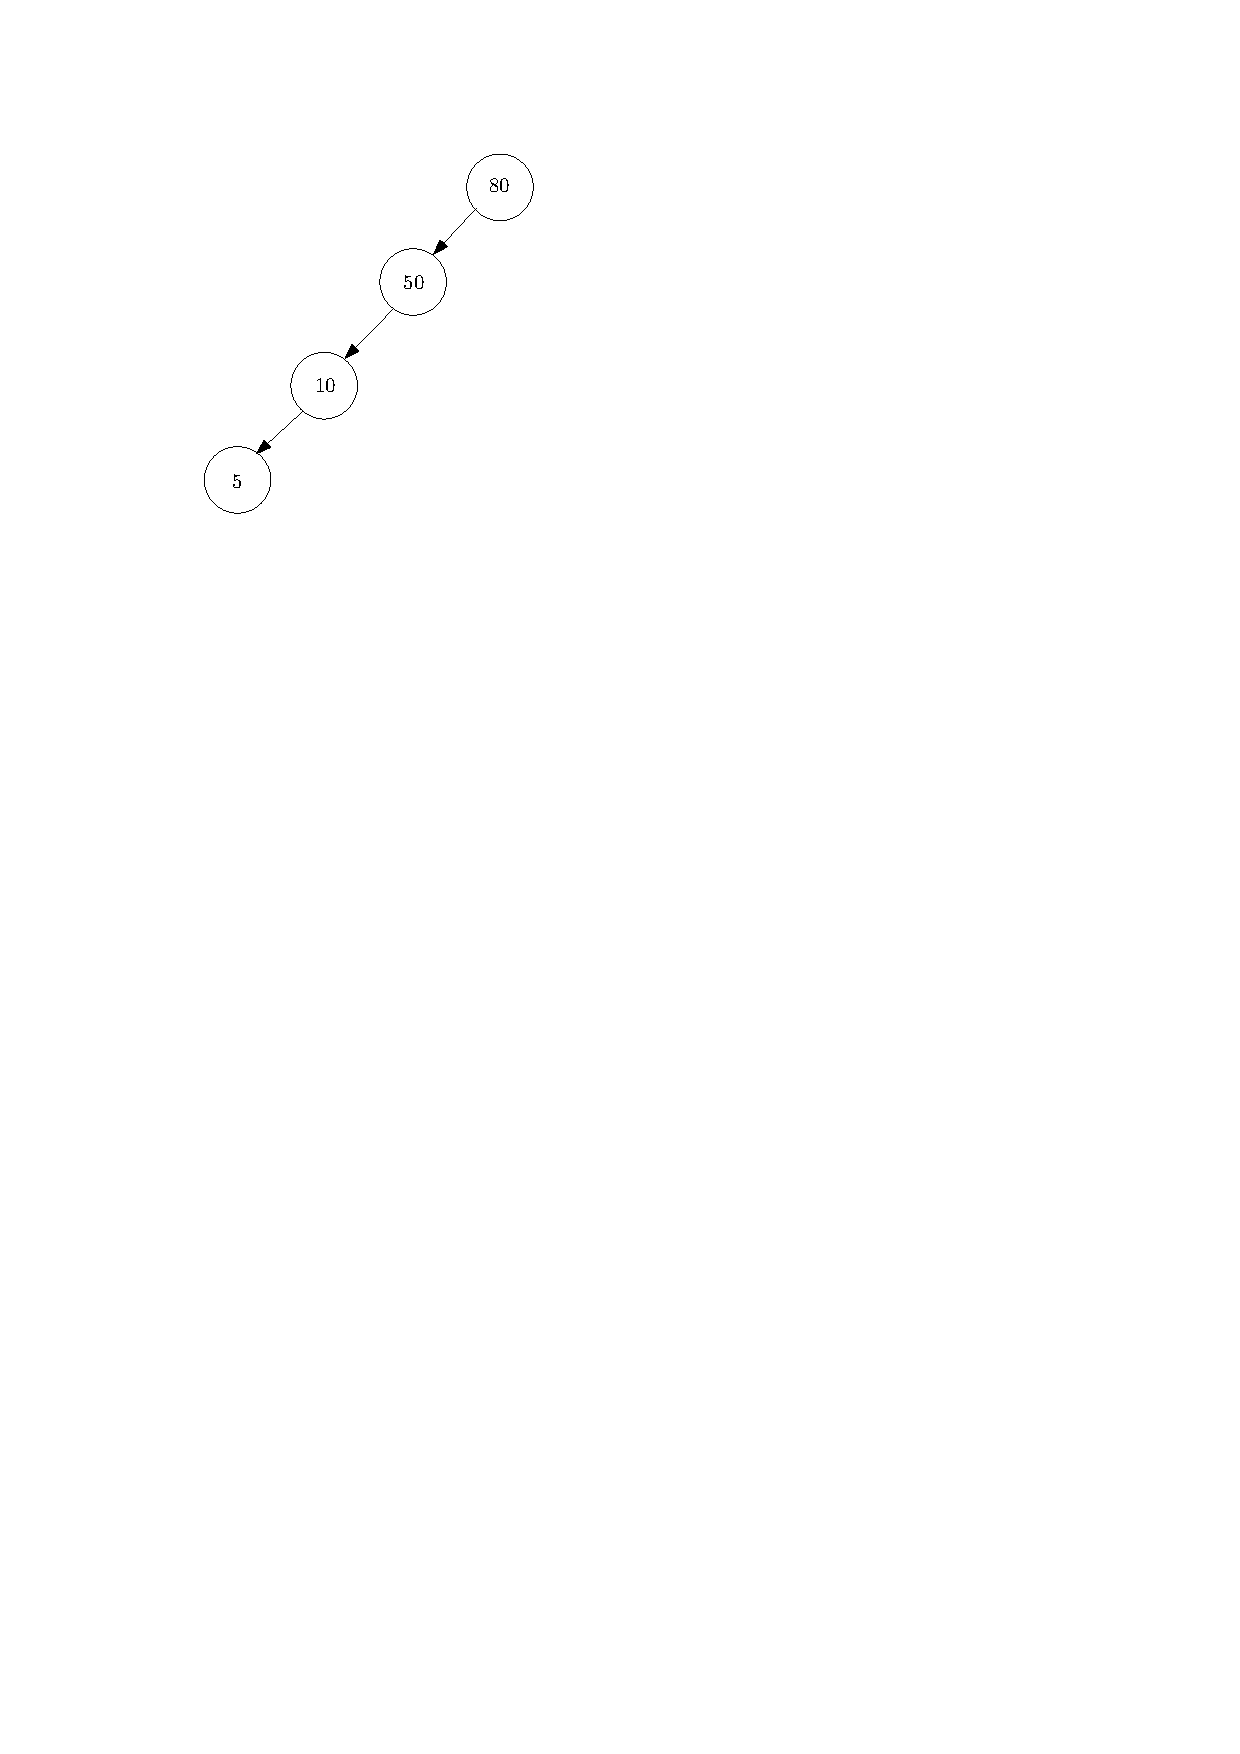
\includegraphics[scale=0.8]{unbalancedbt.pdf}
        \caption{Unbalanced binary search tree}
        \label{fig:unbalancedBT}
    \end{figure}
    \begin{figure}[tbh]
        \centering
        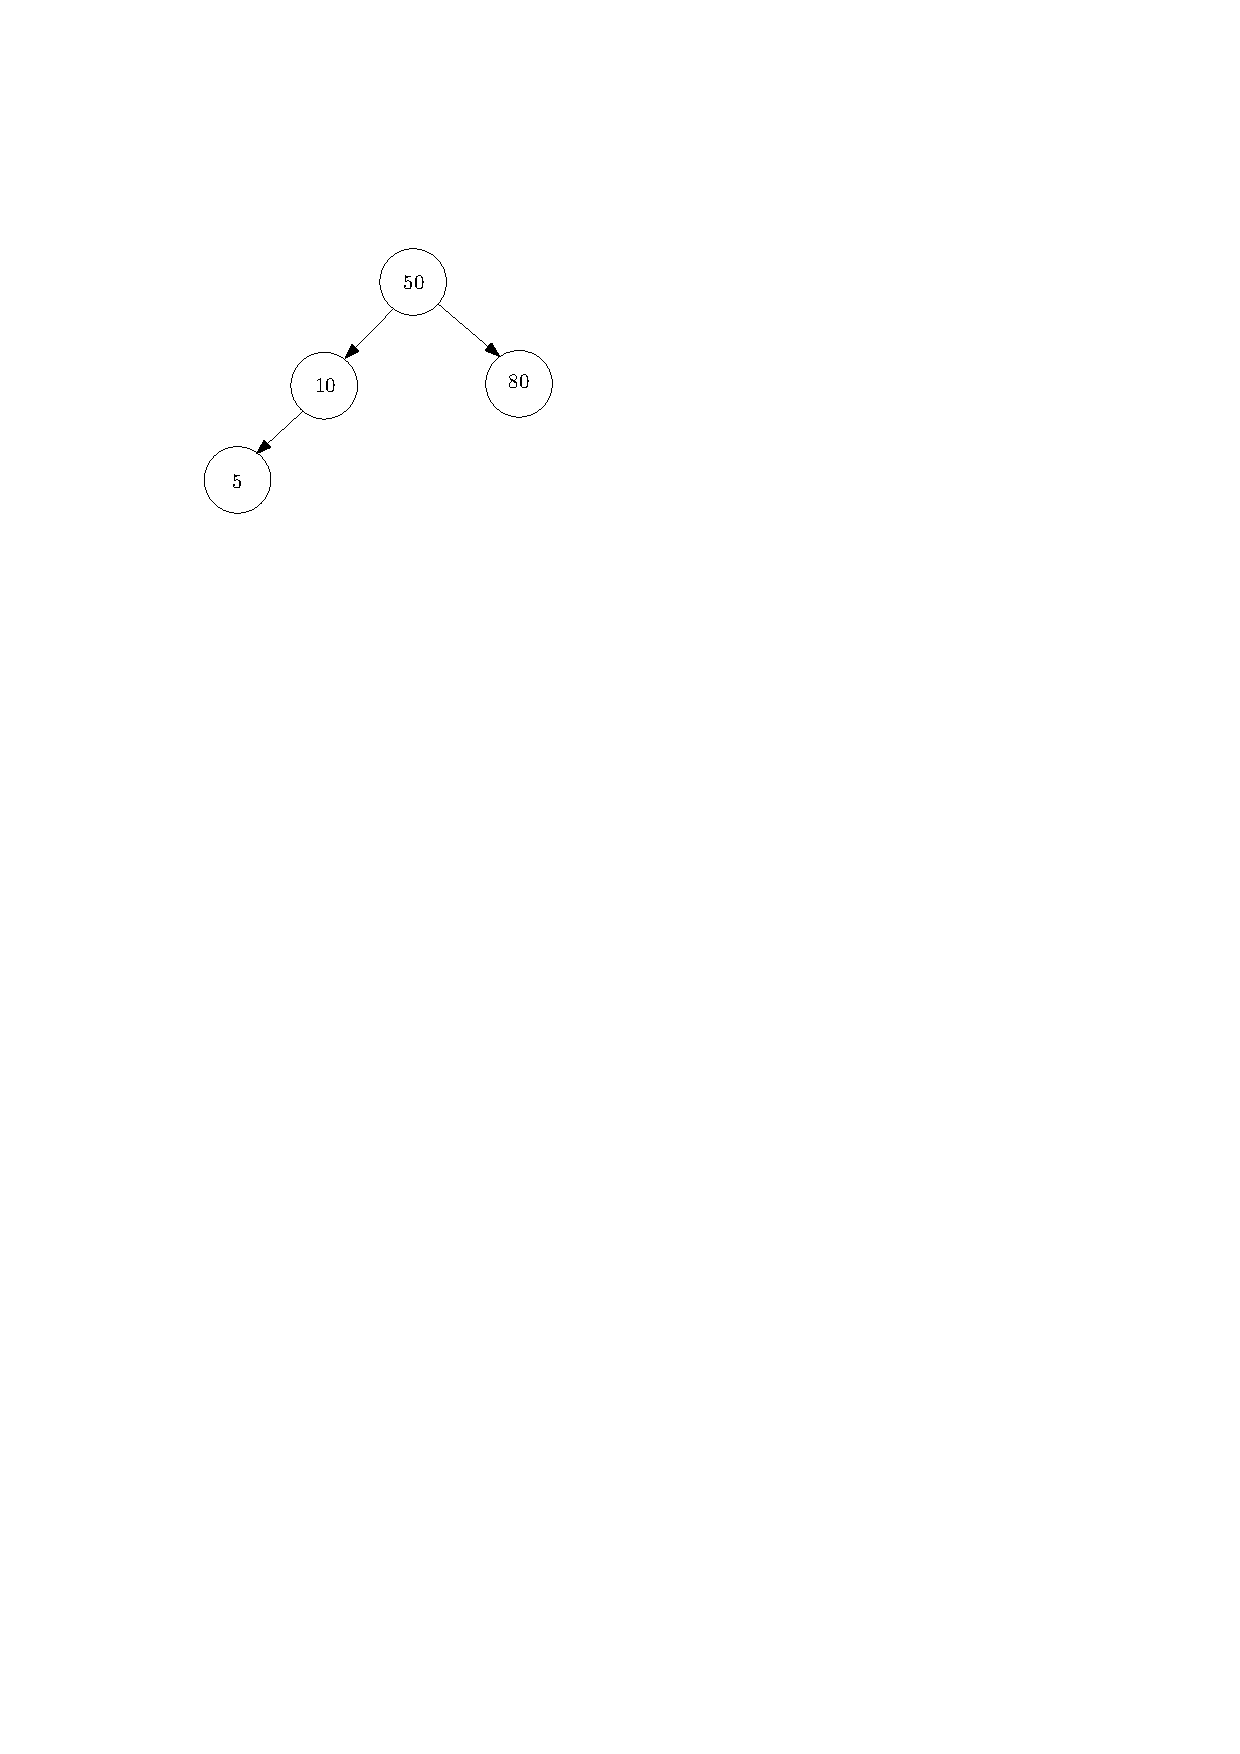
\includegraphics[scale=0.8]{balancedbt.pdf}
        \caption{Balanced binary search tree}
        \label{fig:balancedBT}
    \end{figure}
    
    For example, consider a number of insert operations on a binary search tree as mentioned in Algorithm \ref{Tree:insertion}. The insertions result in a binary search tree corresponding to Figure \ref{fig:unbalancedBT}. If we consider similar $n$ insertions, the cost of search will be $O(n)$ in the worse case. Whereas if we balance the tree like in Figure \ref{fig:balancedBT}, the cost of search can be reduced to $O(\log{n})$.

    Given the probability of access of nodes, cost of search operation in a binary tree can be further improved using an optimal binary search tree instead of a balanced binary tree. Before moving into the optimal binary search tree, let's review dynamic programming.
    
\section{Dynamic Programming}
Dynamic Programming (DP) solves problems by combining the solutions to subproblems. In other words, it is an optimization method over plain recursion. It means that if we have the solutions to some subproblems, we can use them later to solve other problems in a recursive manner. In DP, we solve each subproblem just once and record the solution in a table for later usage. By that, we can save the running time at a cost of using additional memory.

We will look at DP in the context of specific examples including Subset Sum, Knapsack, and Longest Increasing Subsequence. In addition, we introduce two approaches in DP: top-down and bottom-up and elaborate how they differ from each other in terms of implementation while their time complexity is usually of the same order.
\subsection{Subset Sum}
\textbf{ Problem:}  \textit{Given a set of $S$ of $1\leq n\leq 20$ integers,
and a positive integer $x$, is there a subset of $S$ that sums to $x$?}
\paragraph{Example:}
\[
S={17,5,7,15,3,8} \qquad x = 16
\]
Then, the subset $\{5,3,8\}$ of $S$ that sums to 16.

\subsubsection{Top-down Solution: Prune search space as you generate partial solutions}
For the problem, let $\mathbf{SubsetSum(S[i:n], x)}$ be the function to find whether there is a subset of $\mathbf{S[i:n]}$ with sum equal to $x$. $S[i]$ is the $ith$ number of elements in the set.
The problem can be divided into two subproblems:
\begin{itemize}
    \item Include the element $S[i]$, recurse on $i = i+1, x = x-S[i]$.
    \item Exclude the element $S[i]$, recurse on $i = i+1, x = x$.
\end{itemize}


If any of the subproblems return true, then return true.  Because empty set is the subset of any set, when the $x=0$, return true. 

The following is the recursive formula for this problem.

\[
SubsetSum(S[i:n], x) = SubsetSum(S[i+1:n], x);
\]
or
\[
SubsetSum(S[i:n], x) = SubsetSum(S[i+1:n], x-S[i]);
\]
\\
The following is a recursive algorithm that follows the recursive structure mentioned above.
\begin{algorithm}[H]
\caption{Subset-sum: recursive}\label{Subset-sum:recursive}
\begin{algorithmic}[1]
\Function{main}{\null}
\State Initialize $S[1..n]$
\State Initialize $x$
\State\Return{\Call{SubsetSum}{$S, x, 1, n$}}
\EndFunction
\State{\null}
\State \Comment{Returns true iff exists subset within $S[i:n]$ that adds up to $x$;}
\Function{SubsetSum}{$S, x, i, n$}
    \If {$x = 0$}
    \State\Return \Call{true}{}
    \EndIf
    \If {$i>n$ or $x<0$}
    \State\Return \Call{false}{}
    \EndIf
    \If {$S[i]>x$}
    \State \Return {\Call{SubsetSum}{$S, x, i+1, n$}}
    \Else 
    \State\Return \Call{SubsetSum}{$S, x, i+1, n$} or \Call{SubsetSum}{$S, x-S[i], i+1, n$}
    \EndIf
\EndFunction
\end{algorithmic}
\end{algorithm}
The above solution may try all subsets of given set in the worst case. Therefore, time complexity of the above solution is exponential.
\subsubsection{Dynamic Programming Solution}
In the simple recursive solution, every time we calculate the function \Call{SubsetSum}{$S, x, i, n$}, we need to calculate the \Call{SubsetSum}{$S, x, i+1, n$} or \Call{SubsetSum}{$S, x-S[i], i+1, n$} over and over again. So if we can store the \Call{SubsetSum}{$S, x, i+1, n$} before we calculate the \Call{SubsetSum}{$S, x, i, n$}, we need calculate the \Call{SubsetSum}{$S, x, i+1, n$} or \Call{SubsetSum}{$S, x-S[i], i+1, n$} at most one time. Therefore, we create a 2D table $M[0..n][0..x]$ and use it to memoize the return values. The value of $S[i][x]$ will be true if there is a subset of $S[i:n]$ with sum equal to $x$, otherwise false. Finally, we return $S[i][x]$.

The following is a recursive algorithm that follows the recursive structure mentioned above.

\begin{algorithm}[H]
\caption{Subset-sum: DP}\label{Subset-sum:DP}
\begin{algorithmic}[1]
\Function{main}{\null}
\State Initialize $S[1..n]$
\State Initialize $x$
\State Initialize $M[1..n][1..x]$ to $UNDEFINED$ values
\State\Return{\Call{SubsetSumDP}{$S, x, 1, n, M$}}
\EndFunction
\State{\null}
\State \Comment{Returns true iff exists subset within $S[i:n]$ that adds up to $x$}
\Function{SubsetSumDP}{$S, x, i, n, M$}
    \If {$x = 0$}
    \State\Return $M[i][x] = \Call{true}{}$
    \EndIf
    \If {$i>n$ or $x<0$}
    \State\Return \Call{false}{}
    \EndIf
    \If {$M[i][x] \neq UNDEFINED$}
    \State\Return $M[i][x]$
    \EndIf
    \If {$S[i]>x$}
    \State \Return {$M[i][x]=$ \Call{SubsetSumDP}{$S, x, i+1, n, M$}}
    \Else 
    \State\Return $M[i][x]=\Call{SubsetSumDP}{S, x, i+1, n, M}$ {\bf or} $\Call{SubsetSumDP}{S, x-S[i], i+1, n, M}$
    \EndIf
\EndFunction
\end{algorithmic}
\end{algorithm}

In this algorithm, in the worst case, we need calculate the $M[i][x]$ for every $i$ and $x$ at most once, so the worst cost is $O(xn)$.
\subsection{0-1 Knapsack}
\textbf{Problem (0-1 Knapsack)}. \textit{Given a set $S$ of $n$ items, each with its own value $V_i$ and weight $W_i$ for all $1\leq i\leq n$ and a maximum knapsack capacity $C$, compute the maximum value of the items that you can carry. You cannot take fractions of items.}
\paragraph{Example:}
\[\{(V_i,W_i)\} = \{(10,17),(5,7),(3,8),(9,15)\}\qquad C = 16\]
Then, the best value is $9$ in the case of $(V_4,W_4)$.

A simple solution is to consider all subsets of items and calculate the total weight and value of all subsets. This problem is similar to the subset-sum problem. Consider the only subsets whose total weight is smaller than $W$. From all such subsets, pick the subset with the maximum value.
\subsubsection{Recursive Solution}
Like the subset-sum problem, \Call{maxV}{$i,C$} returns the maximum value among items $S[i : n]$ with remaining knapsack capacity of $C$. When $i=1$, that is the initial problem, if the first item is not included in the knapsack, then this problem becomes the problem of finding the maximum value among items $S[2 : n]$ with remaining knapsack capacity of $C$. When the first item is included in the knapsack, then this problem becomes the problem of finding the maximum value among items $S[2 : n]$ with remaining knapsack capacity of $C-W_1$.
To consider all subsets of items, the Knapsack problem can be divided into two subproblems: 
\begin{itemize}
    \item The item is not included in the optimal subset, maximum value obtained by $S[i+1,n]$ and the maximum capacity $C$.
    \item The item is included in the optimal set, maximum value obtained by the value of $ith$ item plus the maximum value obtained by $S[i+1,n]$ and $C-W_i$ .
\end{itemize}
And when the $C\leq 0$, return false, because there is no capacity to store any item. When $i\ge n$, return false, because that is out of the range.

If $W_i>C$ , then $V_i$ cannot be included in the optimal subset and case 1 is the only possibility. Else,  the $V_i$ can be either included in the optimal subset or not included in the optimal subset.

The following is the recursive formula for this problem:
\[
\Call{maxV}{i,C} =
\begin{cases} 
0,  & \mbox{if }i>n \\
0, & \mbox{if }C\leq 0\\
\Call{maxV}{i+1,C},& \mbox{if } W_i>C\\
\max\{\Call{maxV}{i+1,C},V_i+\Call{maxV}{i+1,C-W_i}\},& \mbox{if } W_i \leq C
\end{cases}
\]
The following is a recursive algorithm that follows the recursive structure mentioned above.\\
\begin{algorithm}[H]
\caption{ksnapsack:recursive}\label{ksnapsack:recursive}
\begin{algorithmic}[1]
\Function{main}{\null}
\State Initialize $V[1..n], W[1..n]$ and $C$
\State\Return{$\Call{maxV}{V, W, C, 1, n}$}
\EndFunction
\State{\null}
\Function{maxV}{$V, W, C, i, n$}
    \If {$i>n$ or $C\leq 0$}
    \State\Return $0$
    \EndIf
    \If {$W[i]>C$}
    \State\Return $\Call{maxV}{V, W, C, i+1, n}$
    \Else 
    \State\Return {$\max\{\Call{maxV}{V, W, C, i+1, n},V[i]+\Call{maxV}{V, W, C-W[i], i+1, n}\}$}
    \EndIf
\EndFunction
\end{algorithmic}
\end{algorithm}
\subsubsection{DP solution}
This is similar to the Subset Sum problem. We create a 2D table $M[1..n][1..C]$ and use it to memoize the return values. 

The following is recursive algorithm that  follows the recursive structure mentioned above.

\begin{algorithm}[H]
\caption{ksnapsack:DP}\label{ksnapsack:DP}
\begin{algorithmic}[1]
\Function{main}{\null}
\State Initialize $V[1..n], W[1..n]$ and $C$
\State Initialize $M[1..n][1..C]$ to $UNDEFINED$
\State\Return{$\Call{maxV}{V, W, C, 1, n, M}$}
\EndFunction
\State{\null}
\Function{maxV}{$V, W, C, i, n, M$}
    \If {$i>n$ or $C\leq 0$}
    \State\Return $0$
    \EndIf
    \If{$M[i][C] \ne UNDEFINED$}
    \State \Return{$M[i][C]$}
    \EndIf
    \If {$W[i]>C$}
    \State\Return $M[i][C]=\Call{maxV}{V, W, C, i+1, n, M}$
    \Else 
    \State\Return $M[i][C]=\max\{\Call{maxV}{V, W, C, i+1, n, M}, V[i]+\Call{maxV}{V, W, C-W[i], i+1, n, M}\}$
    \EndIf
\EndFunction
\end{algorithmic}
\end{algorithm}

\subsection{Longest Increasing Subsequence}
The Longest Increasing Subsequence (LIS) problem asks to find the length of the longest subsequence of a given sequence such that all elements of the subsequence are sorted in increasing order. For example, the length of LIS for $A=\{-7, 10, 9, 2, 3, 8, 8, 1\}$ is 4 and $\text{LIS}=\{-7, 2, 3, 8\}$. We employ DP to solve this problem in polynomial time.

Let's consider that $\text{LIS}(i)$ returns the size of the longest increasing subsequence of the array $A[1:i]$. Then, we can write $\text{LIS}(i)$ recursively by deciding whether to add $A[i]$ to the solution of $\text{LIS}(i-1)$ or not. Since we don't know if including/excluding $A[i]$ will block LIS to have longer subsequence later or not, we need to modify this recursion in a little smarter way. To deal with that, we always compare $A[i]$ with all previous $A[j]$ where $j<i$ since $\text{LIS}(i)$ must be the longest increasing subsequence that ends at $i$, i.e.:
\begin{equation*}
\text{LIS}(i)=
\begin{cases}
1 \hspace{5cm} &\text{if} \hspace{0.3cm} i=1 \\
\text{max}
    \begin{cases}
    1 \hspace{4cm} \\
    \text{LIS}(1)+1 \hspace{2cm} \text{if} \hspace{0.3cm} A[i]>A[1]\\
    \text{LIS}(2)+1 \hspace{2cm} \text{if} \hspace{0.3cm} A[i]>A[2]\\
    \text{LIS}(3)+1 \hspace{2cm} \text{if} \hspace{0.3cm} A[i]>A[3]\\
    \ldots \hspace{4cm} \ldots\\
    \text{LIS}(i-1)+1 \hspace{1.45cm} \text{if} \hspace{0.3cm} A[i]>A[i-1]\\
    \end{cases}
    &\text{if} \hspace{0.3cm} i>1
\end{cases}
\end{equation*}
The pseudocode for implementing the above steps is given in the following:

\begin{algorithm}[H]
\caption{Longest Increasing Subsequence}\label{LIS}
\begin{algorithmic}[1]
\Function{main}{\null}
\State Initialize $A[1..n]$
\State Initialize $L[1..n]$ to $UNDEFINED$
\State{$best=0$}
\For{$i =1$ to $n$}
    \State{$current=\Call{LIS}{A, i, L}$}
    \If{$best<current$}
        \State{$best=current$}
    \EndIf
\EndFor
\State \Return{$best$}
\EndFunction
\State{\null}
\Function{LIS}{$A, i, L$} \Comment{Returns longest common subsequence of $A[1..i]$}
\If{$L[i] \ne UNDEFINED$}
    \State \Return{$L[i]$}
\EndIf
\If{$i=1$}
    \State \Return{$L[i]=1$}
\EndIf
\State{$best=1$}
\For{$j =1$ to $i-1$}
    \If{$A[i]>A[j]$}
        \State {$current = \Call{LIS}{A, j, L}+1$}
        \If{$best<current$}
            \State{$best=current$}
        \EndIf
    \EndIf
\EndFor
\State \Return{$L[i]=best$}
\EndFunction
\end{algorithmic}
\end{algorithm}

The complexity to find LIS depends on nested loop and of the order $O(n^2)$. In other words, the entry \Call{LIS}{$i$} takes $O(i)$ time to compute which gives $O(1)+\ldots+O(n)= O(n^2)$ overall complexity.

\subsection{Bottom-up Approach in DP}
The bottom-up approach of DP consists of first looking at the smaller subproblems, and then solving the larger subproblems using the solution to the smaller subproblems. We can think of that as a table filling algorithm where we start by filling out lower cells and then going up. For example, if we need to calculate fifth Fibonacci number, we calculate first, then second then third all the way up to the fifth number. This approach does not use recursion but it consumes more space, since we will iteratively compute all subproblems until we reach the main problem. For example in subset sum problem,  we start by using only the first element. We can either use it or not, so the possible sums are $\{0, A[1]\}$. Now we keep both of these, and also try adding $A[2]$ to each one. We get $\{0, A[1], A[2], A[1]+A[2]\}$. Then we repeat until all of the elements are included. Figure~\ref{fig:bottom-up} illustrates how bottom-up approach is like filling out a table where at each step we need to calculate the applicable underneath cells.

Unlike bottom-up approach, in top-down approach we try to include the first element in the subset, and recursively see if any combination of the rest of elements add up to the rest of the sum. If we don't find a solution, leave out the first element and continue. In other words, we first break the problem into subproblems and then calculate and store values which is the opposite of bottom-up approach where we solve smaller subproblems first, then solve larger subproblems from them.
\begin{figure}[tbh]
\centering
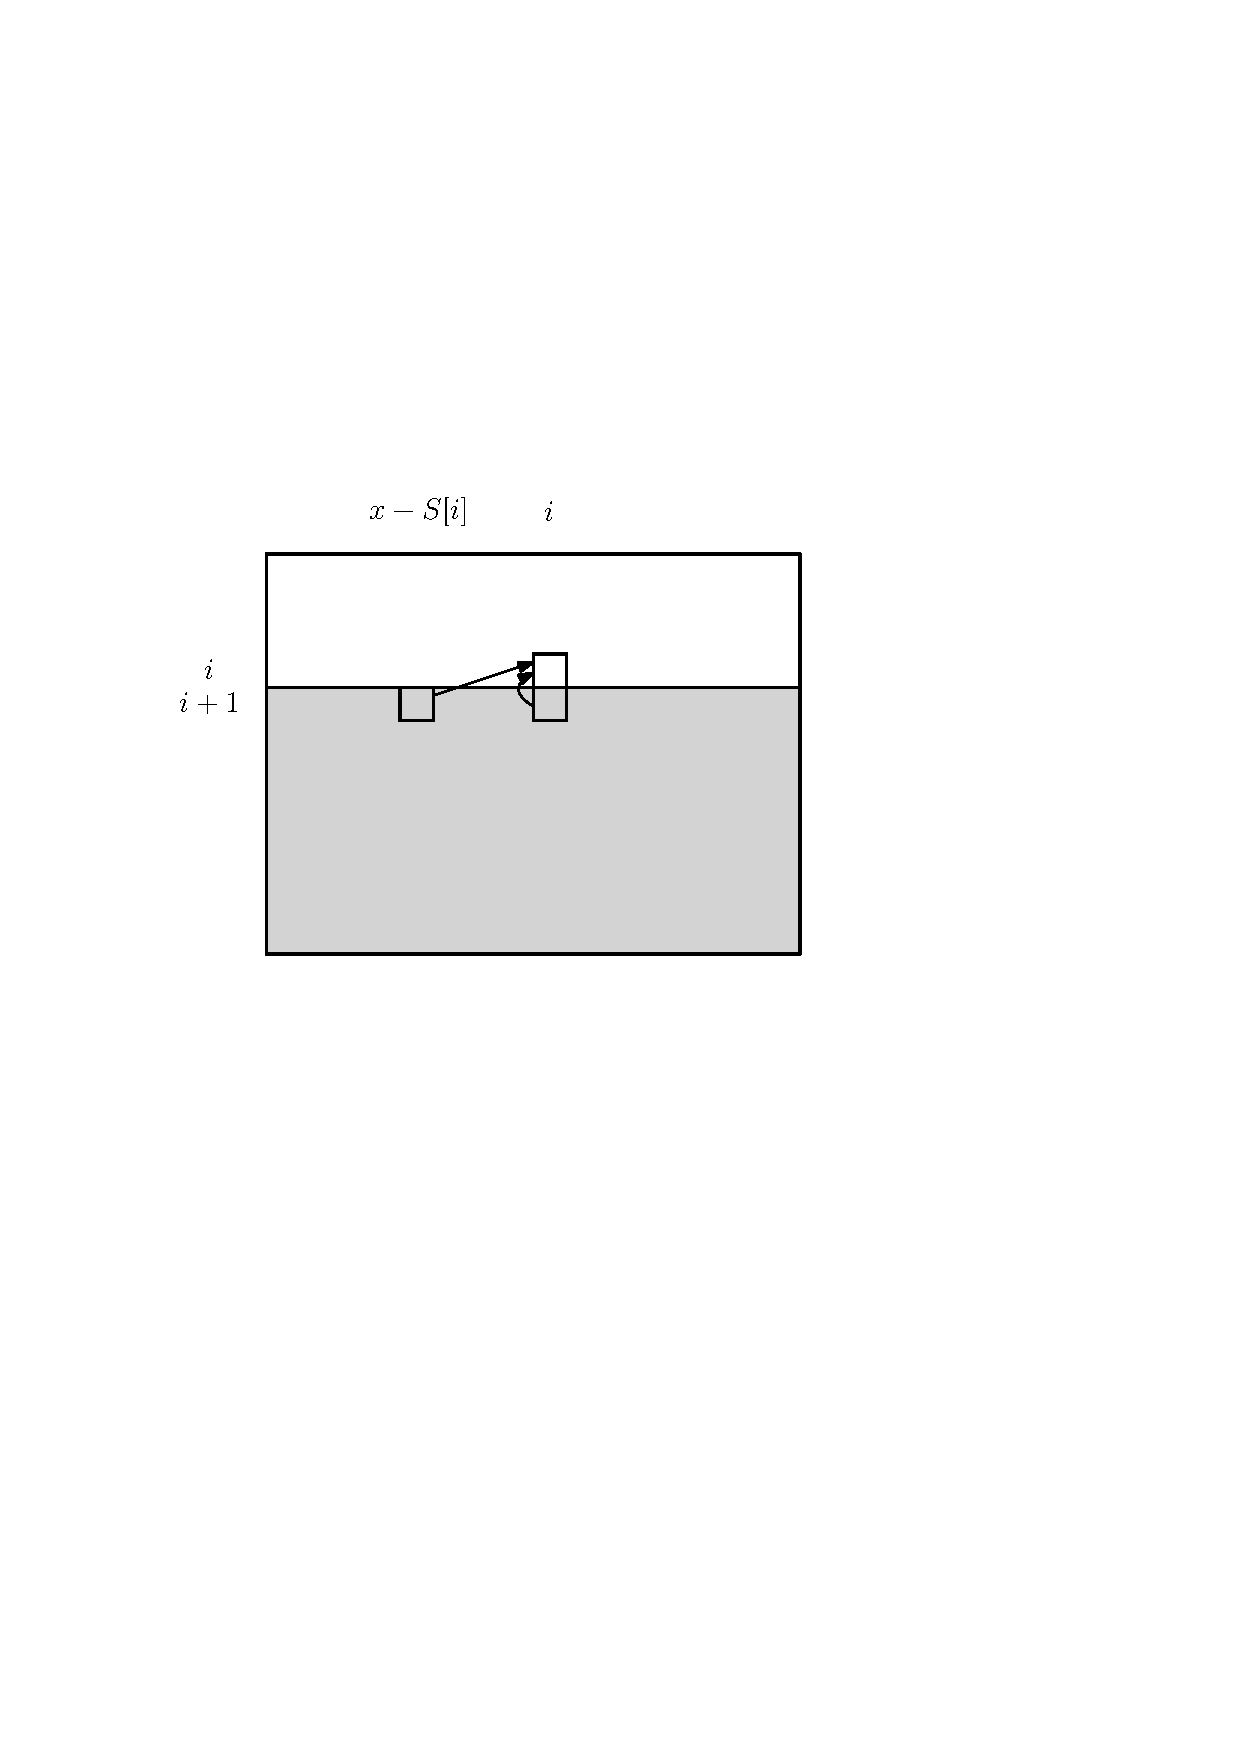
\includegraphics[scale=0.8]{BottomUp.pdf}
\caption{Tabular representation of bottom-up approach for subset sum problem.}
\label{fig:bottom-up}
\end{figure}

The pseudocode for implementation is as follows:
\begin{algorithm}[H]
\caption{Subset-sum: Bottom-Up}\label{Subset-sum:BU}
\begin{algorithmic}[1]
\Function{SubsetSumBottomUp}{$S[1..n], x$}
\State Allocate new $(n+1)\times (x+1)$ array $M[0..n][0..x]$
\For {$i = 0$ to $x$}
\State $M[n][i]=\Call{False}{}$
\EndFor
\For{$i =n$ downto $0$}
    \For{$j=S[i]$ to $x$}
        \State{$M[i][j] = M[i+1][j] \text{ or } M[i+1][j-S[i]]$}
    \EndFor
\EndFor
\State\Return{$M[0][x]$}
\EndFunction
\end{algorithmic}
\end{algorithm}

The time complexity of the above pseudocode is dependent on nested loop which is a function of $|S|$ as the size of the set and $x$ as the desired summation. Therefore, we have $O(|S|\cdot x)$ as the running time for the worst-case which is much better than exponential in the case without DP.

\section{Optimal Binary Search Tree}
        The problem of a Optimal Binary Search Tree can be rephrased as:

    \emph{Given a list of $n$ keys ($A[1, ..., n]$) and their frequencies of access ($F[1, ..., n]$), construct a optimal binary search tree in which the cost of search is minimum.}
    
    We will start with a list of keys in a tree and their frequencies. Now to find the best binary tree with minimum cost to search in the tree, we can create all possible binary trees out of our list of keys and find the cost of searching items in those binary trees and pick one of the best binary tree as our optimal binary search tree.
    
    Further we can use divide and conquer strategy to solve our problem. Note that if we have an optimal binary tree then at any node of that tree, it should have an optimal binary search tree on its left child tree and also an optimal binary search tree on its right child tree. Thus we can break our original problem into two sub problems and use same method to solve for those sub problems.
    
    Our objective for this problem is to find the tree with minimum cost for searching. So we can use the cost of searching keys in the tree as our objective function for our recursive function. And before we move on to our recursive solution, let's look at the cost of searching a binary search tree in detail. 
    \begin{figure}[tbh]
        \centering
        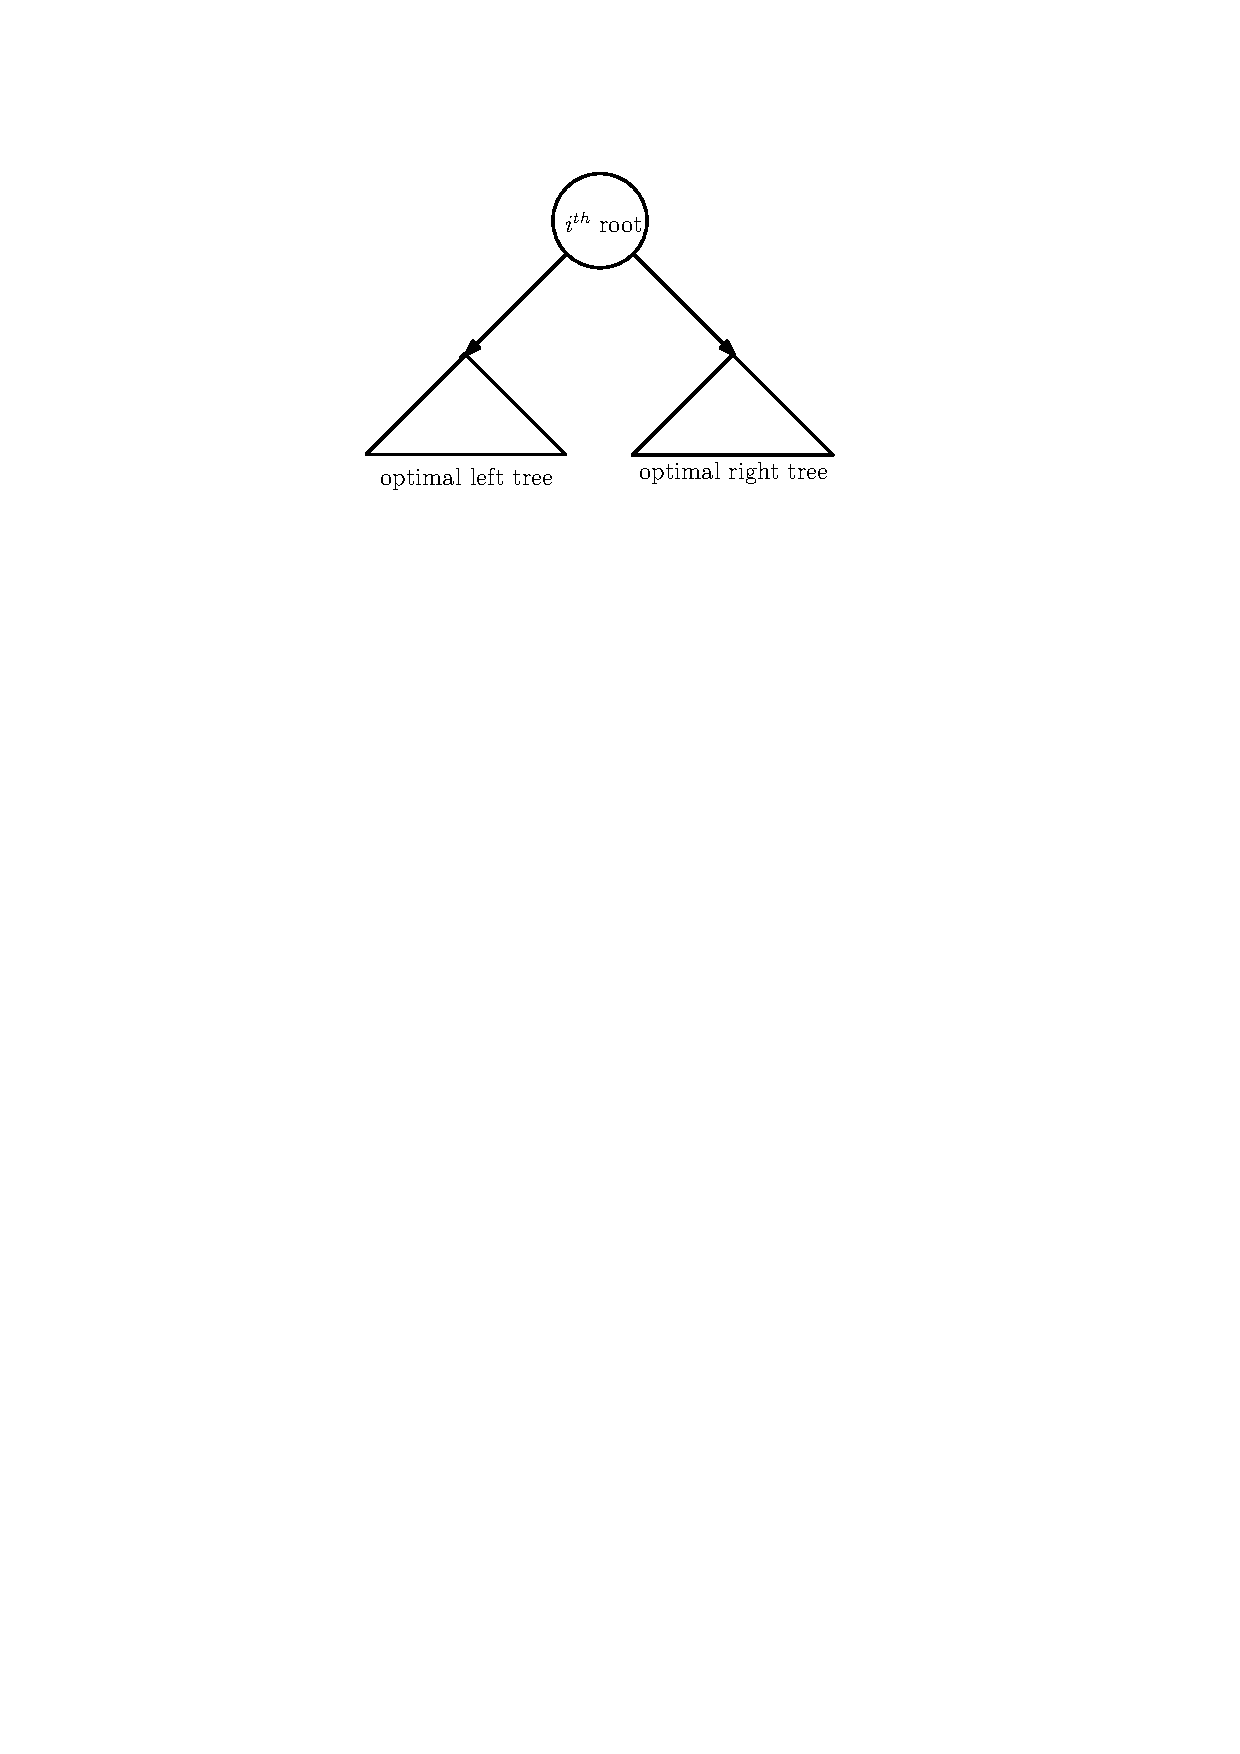
\includegraphics[scale=1]{optimalBST.pdf}
        \caption{Dividing Optimal Binary Search Tree problem to sub problems}
        \label{fig:optimalBST}
    \end{figure}
    
    Given any binary search tree $T$, the total cost of searching can be calculated by calculating sum of product of frequencies of the nodes ($f[v]$) and depth of the nodes in the tree ($d[v]$).
    \begin{equation}
        cost_{total} = \sum_{v \in T} f[v]\cdot d[v]
    \end{equation}
    
    Thus, the problem of finding the cost of searching the binary search tree can be solved recursively as follows (see Figure \ref{fig:optimalBST}) for reference).

For the left optimal tree ($T_{left}$), the cost of searching in the left optimal subtree is given by: 
    \begin{equation}
        cost_{left} = \sum_{v \in T_{left}} f[v]\cdot d[v]
    \end{equation}
    Similarly for right optimal subtree ($T_{right}$), the cost of searching in the right optimal subtree is given by:
    \begin{equation}
        cost_{right} = \sum_{v \in T_{right}} f[v]\cdot d[v]
    \end{equation}
    Now, if we combine left and right optimal trees with the root node just like in Figure \ref{fig:optimalBST}, the depth for nodes in left and right subtree are increased by 1 and the updated cost for left and right subtree is given by: 
    \begin{center}
        \begin{align*}
            cost_{left\_new} &= \sum_{v \in  T_{left}} f[v]\cdot (d[v] +1)\\
            &= \sum_{v \in  T_{left}} f[v]\cdot d[v] + \sum_{v \in  T_{left}} f[v]\\
            &= cost_{left} + \sum_{v \in  T_{left}} f[v]\\
            \\
            cost_{right\_new} &= \sum_{v \in  T_{right}} f[v]\cdot  (d[v] +1)\\
            &= cost_{right} + \sum_{v \in  T_{right}} f[v]\\
        \end{align*}
    \end{center}
    And, the final cost is sum of the cost of search on right, cost of search on left and the number of times we search for the root node (equal to the frequency of the key in the root node).
    \begin{center}
        \begin{align*}
            cost_{total} &= cost_{left\_new} + cost_{right\_new} + f[root]\\
            &= \left(cost_{left} + \sum_{v \in  T_{left}} f[v] \right)+ \left(cost_{right}   + \sum_{v \in  T_{right}} f[v]\right) + f[root] \\
            &= cost_{left} + cost_{right}   + \left(\sum_{v \in  T_{left}} f[v] + \sum_{v \in  T_{right}} f[v] + f[root]\right)
        \end{align*}
    \end{center}
    
    For our implementation with array of keys and frequencies, if we sort the keys and frequencies based on keys then we can say that if we pick any of the array element as a root node for our tree, the sub-array in the left of the key can be used as nodes for left binary sub-tree and the sub-array in the right of the key can be used as nodes for right sub-tree. For example if we want to create tree out of array that is bound by indices $L$ and $R$ with root node at index $i$, the cost of searching in the tree can be obtained using: 
     \begin{center}
        \begin{align*}
            cost_{total} &= \sum_{v=L}^{i-1} f[v]\cdot d[v] + \sum_{v = i + 1}^{R} f[v]\cdot d[v] + \left(\sum_{v=L}^{i-1} f[v] + \sum_{v = i + 1}^{R} f[v] + f[i]\right)\\
            &= \sum_{v=L}^{i-1} f[v]\cdot d[v] + \sum_{v = i + 1}^{R} f[v]\cdot d[v] + \sum_{v=L}^{R} f[v]\\
            &= cost_{left} + cost_{right} + \sum_{v=L}^{R} f[v]\\
        \end{align*}
    \end{center}
So using the cost function we can implement recursive solution for the problem as:

\begin{algorithm}[H]
\caption{\Call{Main}{}}\label{Main}
\begin{algorithmic}[1]
\State Sort $A[1..n]$ and $F[1..n]$ by the keys
\State \Return \Call{findOptimalCost}{$A$, $F$, $1$, $n$}
\end{algorithmic}
\end{algorithm}

\begin{algorithm}[H]
\caption{\Call{findOptimalCost}{$A$, $F$, $left$, $right$}}\label{findOptimalCost}
\begin{algorithmic}[1]
\State $best = +\infty$
\For{$i = left$ to $right$} \Comment {try each as the root}
    \State $cost_{left} = \Call{findOptimalCost}{A, F, left, i-1}$
    \State $cost_{right} = \Call{findOptimalCost}{A, F, i+1, right}$
    \State $cost_{total} = cost_{left} + cost_{right} + \sum_{v=left}^{right} F[v]$
    \If {$cost_{total} < cost_{best}$}
      \State $best = cost_{total}$
    \EndIf
\EndFor\\
\Return $best$
\end{algorithmic}
\end{algorithm}

\end{document}
